% !TEX root = ../DP_Vik_Tomas_2013.tex
\chapter{Implementace}
Pro lepší přestavu bude nejdříve zběžně popsán způsob, jakým se všeobecně sestavuje aplikace ve frameworku Ruby on Rails. Následně se bude kapitola věnovat detailněji implementaci napojení aplikace na srovnávač Heureka.cz, implementací získávání aktuálních cen a jejich zpracování do grafu a na konci kapitoly bude ukázka implementovaných obrazovek aplikace.

\section{Standardní rozvržení aplikace v Ruby on Rails}
Jak již bylo řečno v kapitole \ref{sec:ror}, aplikace upřednostňuje konvenci před konfiguraci, což na jednu stranu znamená minimum konfigurace aplikace, na druhou stranu to znamená že má vývojář přesně dané postupy jak v implementaci něčeho dosáhnout. Framework je postaven na návrhovém vzoru MVC a to také implementaci rozděluje na tři významné části.

\subsection{Model}
Model reprezentuje informace v aplikaci a pravidla jak s nimi zacházet. Což se dá interpretovat také jako mechanismus zapisování a čtení databáze a pravidla tohoto zápisu/čtení. Model je v Rails řešen pomocí knihovny Active Record. Ta poskytuje nad každým objektem modelu velkou škálu funkcí ketré manipulují přímo s databází. Každá modelová třída musí dědit od |ActiveRecord::Base|. Na schématu \ref{fig:model-diagram} jsou vidět všechny modelové třídy ve výsledné aplikaci. Každý model v Rails má v příslušené tabulce v databázi ještě dva sloupce |create_at| a |updated_at| jejichž hodnoty se automaticky nastavují při vytvoření/upravení záznamu.

\begin{figure}[htb]
\begin{center}
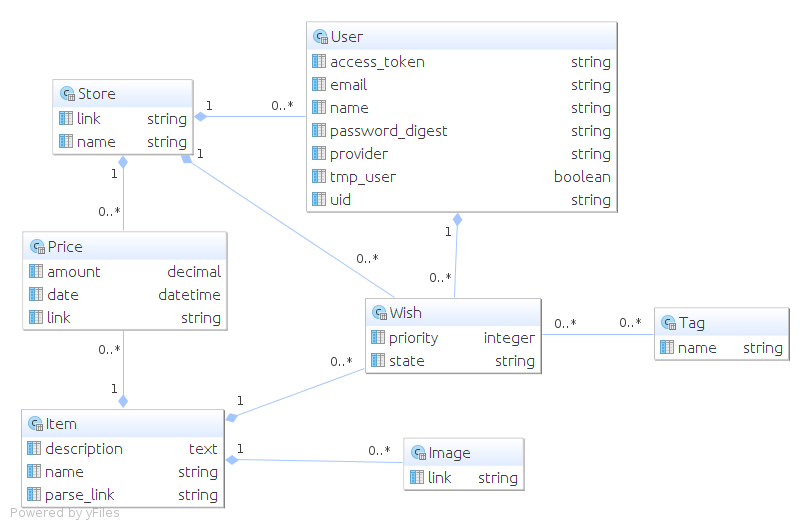
\includegraphics[width=120mm]{./pictures/model-diagram.png}
\caption{Digram tříd v modelu aplikace}
\label{fig:model-diagram}
\end{center}
\end{figure}

\subsection{Controller}
Controller je v Rails třída, která dědí od třídy |ActionController::Base|. Tato třída má na starosti zpracování HTTP dotazů. Pokud přijde dotaz, framework se pokusí v routes souboru\footnote{Konfigurační soubor, ve kterém jsou nastaveny pro každou validní URL odpovídající controllery a jejich metody.} najít vhodný controller a jeho metodu kterou poté zavolá. Controller má mimo jiné přístup k parametrům se kterými byl proveden HTTP dotaz a k session proměnné.

Dále je v Rails aplikacích standardem, že existuje controller, který se nazývá |ApplicationController| a od něj dědí všechny ostatní controllery. Tak je tomu i ve výsledné aplikaci.

V následující ukázce je kus kódu největšího controlleru výsledné aplikace |WishesController|. Konkrétně metoda, která se volá po odeslání formuláře na přidání přání.

\lstset{language = ruby, style=custom}
\begin{lstlisting}
class WishesController < ApplicationController

#....... kod vynechan

  # POST /wishes
  # POST /wishes.json
  def create
    #ziskame prani pro id z parametru
    @wish = Wish.new(params[:wish])
    #z retezce ziskame stitky
    tags = Tag.parse_tags(params[:tags])
    @wish.tags = tags
    @wish.user = current_user
    #inicializujeme prioritu prani
    @wish.initialize_priority(params[:user_priority].to_d)
    respond_to do |format|
      format.html { redirect_to wishes_path, notice: :success }
      format.json { render json: @wish, status: :created, location: @wish }
    end
  end

#....... kod vynechan

end
\end{lstlisting}

\subsection{View}
View reprezentuje uživatelské rozhranní aplikace. V Rails je view řešeno pomocí HTML souborů, do kterých jsou vloženy kusy Ruby kódu. View poskytují data klientskému prohlížeči.

View je vykreslován controllerem a má také k dispozici všechna data, která má k dispozici controller. Proto je snadné předávat do view data získaná v controllru.

Následuje ukázka kódu view, který má ve výsledné aplikace na starost vykreslení seznamu štítků v levém panelu.

\lstset{language = html, style=custom}
\begin{lstlisting}
<div id="tag-overview" class="sidebar-nav">
  <div class="well">
    <ul class="nav nav-stacked nav-pills">
      <li class="nav-header">Stitky</li>
      <% @main_page_tags.each_with_index do |tag, index| %>
          <li <%= 'class=overflow' if index > 4  %>>
            <a href="/wishes/bytag/<%= tag.name %>">
              <%= truncate(tag.name, length: 12) %> <%= raw(ApplicationHelper.badge(tag.wish_count(current_user.id))) %>
            </a>
          </li>

      <% end %>
      <% if @main_page_tags.size > 4 %>
          <li><a id="more-tags-button" class="more" href="#"><i class="icon-chevron-down"></i>Vice</a></li>
      <% end %>
    </ul>
  </div>
</div>
\end{lstlisting}

\section{Napojení výsledné aplikace na srovnávač Herueka.cz}
Jako zdroj dat pro aplikaci je využit server pro srovnávaní cen \textbf{Heureka.cz} a způsob získávání dat z tohoto serveru je \textbf{Web scraping}. Pro usnadnění získávání dat z webových stránek je použita knihovna Nokogiri\footnote{\url{http://nokogiri.org/}}.

Získávání dat spočívá v dotazování na specifické URL serveru. To má vždy stejnou podobu, například získání dokumentu s výsledky hledání produktu vypadá následovně:

\lstset{language = ruby, style=custom}
\begin{lstlisting}
doc = Nokogiri::HTML(open("http://www.heureka.cz/?h[fraze]=#{heureka_term}"))
\end{lstlisting}

\noindent kde |heureka_term| je vyhledáváný výraz.

V takto získaném dokumentu je snadné hledat jednotlivé elementy pomocí css selektorů (viz. \ref{sec:css-selektor}). A číst obsah takto získaných elementů pomocí metody. Následuje ukázka kódu\footnote{Pro přehlednost bylo z ukázky odebráno přiřazení získaných dat.} na získání produktů z vyhledávání provedeného předchozím příkazem:

\begin{lstlisting}
products = doc.css('#content #search .product')
products.each do |product|
  image_link = product.css('.foto img').first['src']
  description_document = product.css('.desc p.small').first
  if description_document
    search_item.description = description_document.content
  end
  item_link = product.css('div h2 a').first
  #nazev produktu
  name = item_link.content
  #odkaz na tento produkt, ze ktereho se prani ziska
  parse_link = item_link['href']
  #pokud odkaz nevede na heureku => neslo by parsovat dalsi data
  next if search_item.parse_link.include? 'exit'
  price_from_to = product.css('.wherebuy .price a.pricen').first.content
  price_from = price_from_to.split('-').first.gsub(/[^0-9]/i, '')
  price_to = price_from_to.split('-').last.gsub(/[^0-9]/i, '')
end
\end{lstlisting}

Základními metodami naimplementované knihovny pro získávání dat ze serveru Heureka.cz jsou:

\begin{itemize}
\item |search_term(term, limit)| - vrátí vyhledané produkty, tyto produkty nejsou ještě vloženy do databáze, každý vyhledaný produkt obsahuje URL, ze kterého je možné jeho data získat
\item |parse_item(item_url)| - je volána při přidávání přání s novým produktem, získa z dané URL produkt, uloží všechny jeho informace do databáze a vrátí jej
\item |get_prices(item)| - volá se při vytváření nového přání a poté periodicky každý den. Získá ceny ze všech obchodů, ve kterých se produkt z parametru prodává.
\end{itemize}

Při implementaci získávání dat metodou Web Scraping bylo nejobtížnější ošetřit všechny možné podoby stránek, které server vrací. Např. videa v galerii obrázků, žádný popis nebo obrázek produktu apod.

\section{Získávání cen a sestavování grafu vývoje ceny}

\section{Výsledné grafické uživatelské rozhranní.}
